\section{RTC::Multi\-Mode\-Component\-Action Interface Reference}
\label{interfaceRTC_1_1MultiModeComponentAction}\index{RTC::MultiModeComponentAction@{RTC::MultiModeComponentAction}}
Execution\-Semantics::Multi\-Mode\-Component\-Action interface.  


{\tt import \char`\"{}RTC.idl\char`\"{};}

Inheritance diagram for RTC::Multi\-Mode\-Component\-Action::\begin{figure}[H]
\begin{center}
\leavevmode
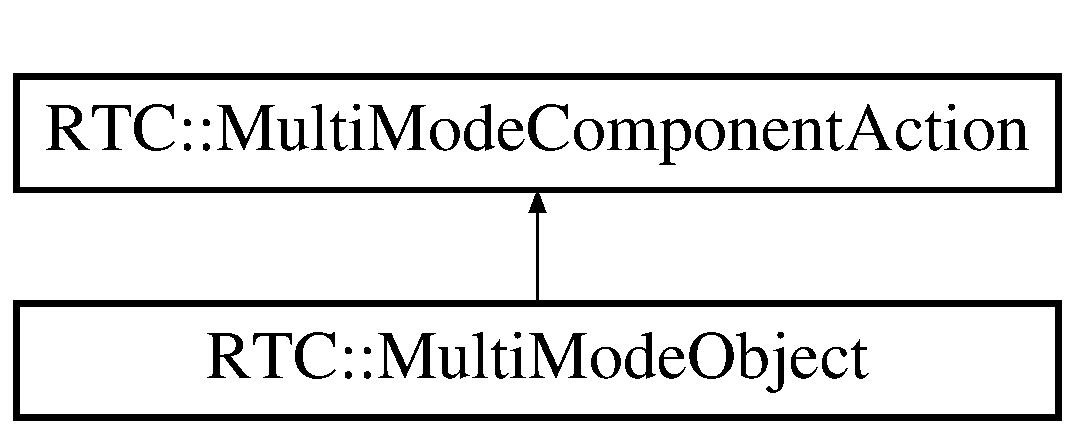
\includegraphics[height=2cm]{interfaceRTC_1_1MultiModeComponentAction}
\end{center}
\end{figure}
\subsection*{Public Member Functions}
\begin{CompactItemize}
\item 
{\bf Return\-Code\_\-t} {\bf on\_\-mode\_\-changed} (in {\bf Lightweight\-RTObject} comp, in {\bf Unique\-Id} ec\_\-id)
\end{CompactItemize}


\subsection{Detailed Description}
Execution\-Semantics::Multi\-Mode\-Component\-Action interface. 



\subsection{Member Function Documentation}
\index{RTC::MultiModeComponentAction@{RTC::Multi\-Mode\-Component\-Action}!on_mode_changed@{on\_\-mode\_\-changed}}
\index{on_mode_changed@{on\_\-mode\_\-changed}!RTC::MultiModeComponentAction@{RTC::Multi\-Mode\-Component\-Action}}
\subsubsection{\setlength{\rightskip}{0pt plus 5cm}{\bf Return\-Code\_\-t} RTC::Multi\-Mode\-Component\-Action::on\_\-mode\_\-changed (in {\bf Lightweight\-RTObject} {\em comp}, in {\bf Unique\-Id} {\em ec\_\-id})}\label{interfaceRTC_1_1MultiModeComponentAction_RTC_1_1MultiModeObjecta6}




The documentation for this interface was generated from the following file:\begin{CompactItemize}
\item 
{\bf RTC.idl}\end{CompactItemize}
